\subsection{Integrated deduplication, caching, and Docker registries}
\label{sec:design}

%\sysname\ performs file-level deduplication for a Docker registry.
%
\begin{figure*}[t]
	\centering
		%\begin{minipage}{0.225\textwidth}
			\centering
			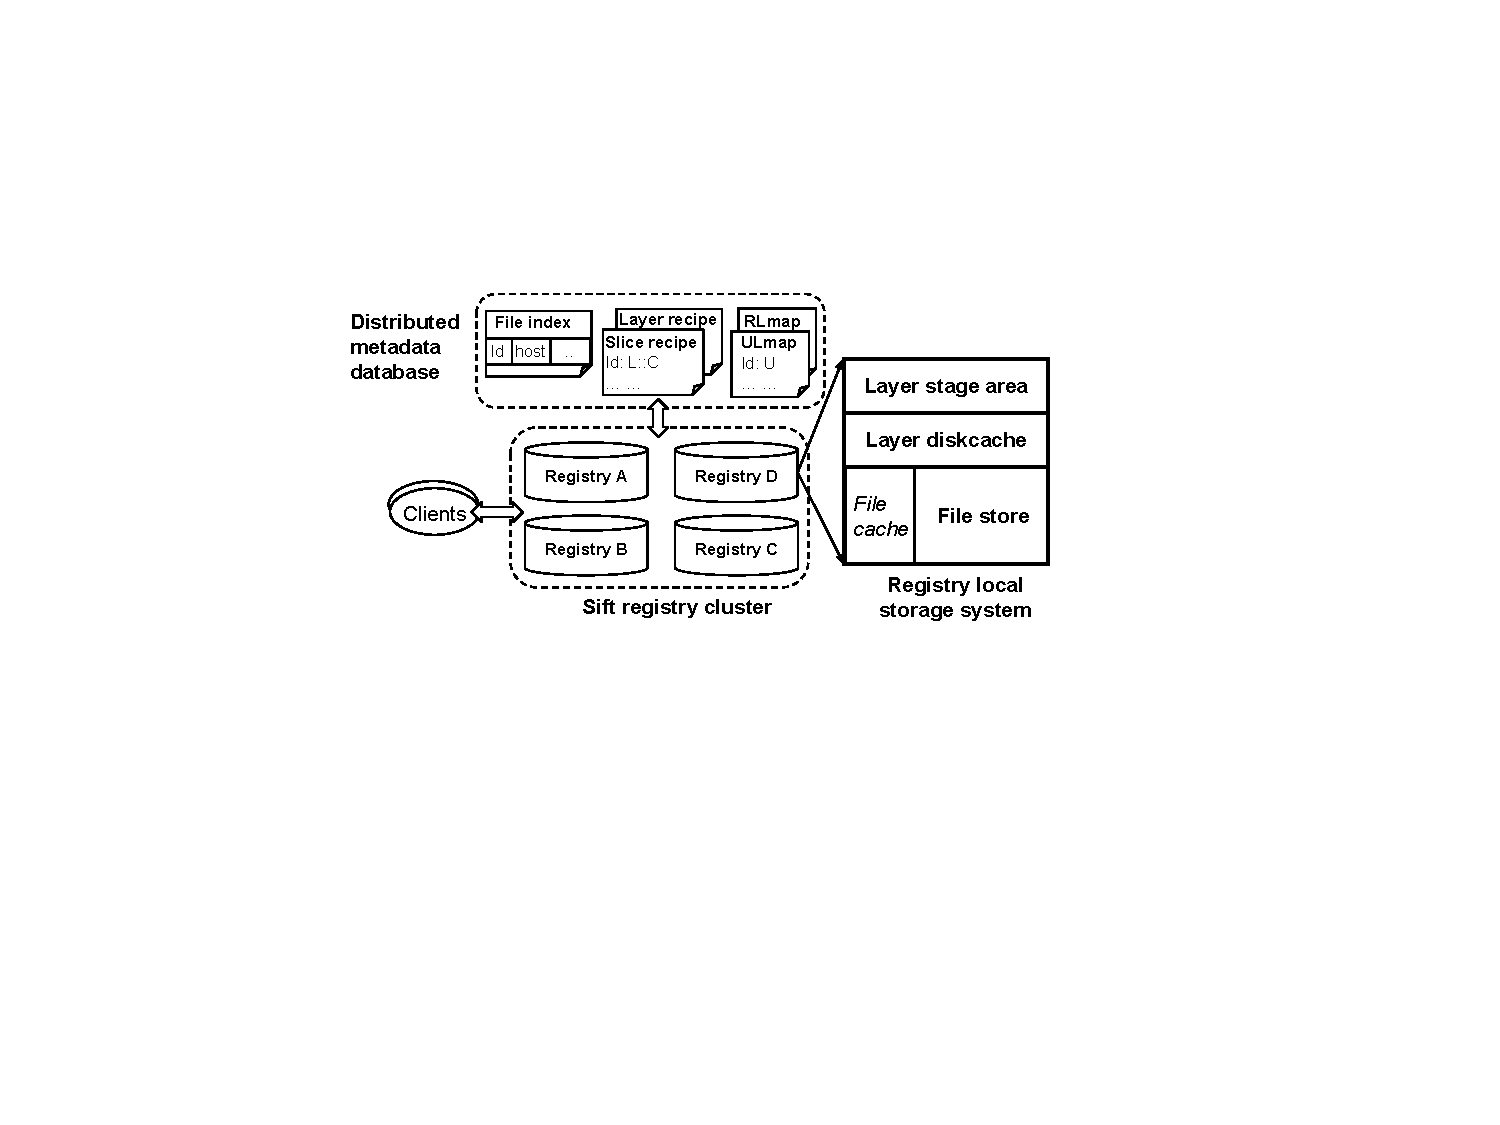
\includegraphics[width=0.9\textwidth]{graphs/sys-architecture.pdf}
%\vspace{-4pt}
			\caption{Architecture of \sysname.}
			%\label{fig:ref_count}
		%\end{minipage}
%	\begin{minipage}{0.225\textwidth}
%		\centering
%		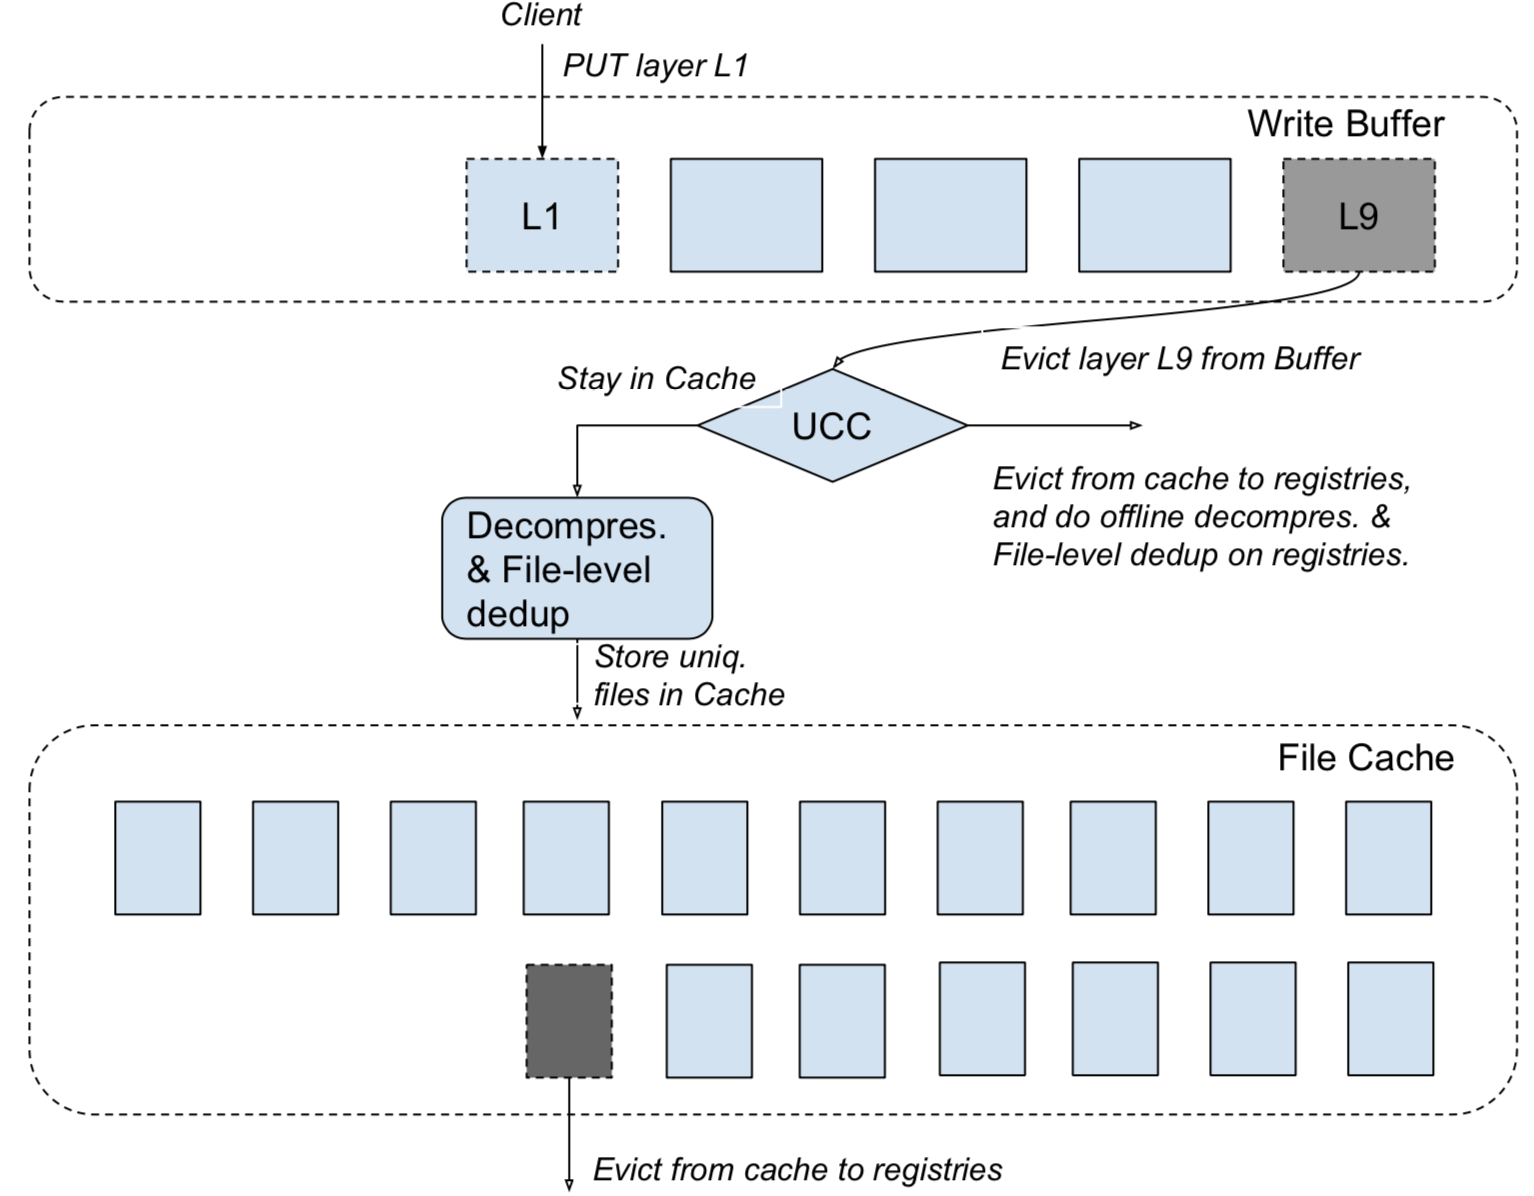
\includegraphics[width=1\textwidth]{graphs/slimmer-cache.png}
%		\caption{CDF of compress. and uncompress. layer size.}
%		\vspace{-3pt}
		\label{fig:sys-overview}
%\vspace{-4pt}
%	\end{minipage}
\end{figure*}

%We designed \sysname\ so that the interface between the Docker clients and the
%registry remains unchanged.
%
%As such, no modifications to the Docker clients are needed.
%
%Below we describe how \sysname\ handles layer pushes and
%pulls at the registry side.
%
%For the sake of this paper, we explain only the main steps omitting smaller
%details.

\sysname~seamlessly integrates the management of cache, deduplication on backend storage (called backend dedupe storage), and Docker registries.
Traditionally, caches are placed as close to the requesting client as possible, 
such caches are known as proxy caches, or web/HTTP caches for the short-lived storage of 
frequently requested/accessed data to reduce the server's lag. 
They are typically implemented in an regional ISP or within a corporate network.
Deduplication methods are implemented on remote backend storage servers, and
transparently remove duplicates from the incoming data stream and restore the data for read requests. 
Docker registry is a web server that serves docker pull and docker push requests.
Although Docker registry is a layer-level content addressable storage system holding all the images,
it delegates storage to drivers which interact with either a local file system or a remote cloud storage like S3, Microsoft Azure, OpenStack Swift, and Aliyun OSS.
Intuitively, registries can be deployed as a proxy cache to host frequently requested layers to speedup image pulls and improve performance 
while the backend cloud storage can leverage deduplication to save storage space.
However, there are several unique problems concerning the integration of caching and deduplication to the unique Docker registries workload: \textbf{compressed layers}. 

First, for caching layers, PULL layer requests are difficult to predict because layer reuse time is very long. 
We observed that, on average, around half of layers' reuse time is longer than 4 hours which means 
that if we cache a layer, we might need to wait hours to get a hit on that layer.
This is because when a user pulls an image from registry, the Docker daemon on the requesting host will only pull the layers that are not stored locally. 
Moreover, we have to consider that users might deploy their applications on different machines, so it's not easy to predict 
when a user will access which layers.
Ali Anwar et. al, proposed a prefetching method~\cite{dockerworkload} based on the push-pull relationship: 
when there is a PUT layer request directly followed by a GET manifest request, a GET layer request will most probably follow.
However, based on our trace analysis, only half of PULL layer requests have a precedent PUT layer request within the trace collecting duration of 75 days. 
This means that,
after a user pushes a layer to the registry, it takes a few days, weeks, or even months for a user to make a PULL requests.

Second, for deduplicating compressed layers, 
the layers should first be decompressed then the uncompressed data undergoes a file-level deduplication. 
While for restoring a layer, the layer's
containing files should all be fetched from wherever they reside, as they are likely to be scattered across multiple servers, 
and compressed together, which causes a considerable overhead on pull layer requests performance.

To meet these challenges, we propose a new registry design featuring a user behavior based cache to reduce the performance degradation caused by deduplication on backend storage system (Figure~\ref{fig:sys-overview}).
Based on our observation, user active time is easier to predict as shown in Figure~\ref{fig:reusetime}.
Therefore, our cache design considers user behavior, including when a user will be active later, which is decisive for layer evictions from the cache.

Considering layer sizes around several megabyte on average~\cite{dockerworkload}, 
a small main memory cache cannot accommodate many active users' layers.
To address this issue, we couple main memory and flash memory to provide separate caching for layers and \emph{deduped} files, respectively, named \emph{layer buffer} and \emph{file cache}.
When handling cache evictions, we first evict inactive users' layers from the layer buffer and \emph{deduped} the layer, then store the \emph{deduped} file into file cache (detailed in \cref{sec:design_operations}). 
%the following operations: decompressing each evicted layer and comparing its containing files with the files that are already 
%stored in the file cache, eliminating duplicate files, that is, only storing the unique files on flash storage.
Consequently, flash memory is facilitating the logical accommodation of more layers when compared to only naively caching layers.
When a user requests a layer not present in the layer buffer, the request will be forwarded to the file cache (detailed in~\cref{sec:design_operations}). 
%More specifically,  

When there is PULL layer request miss on both layer buffer and file cache, the request will be forwarded to the backend dedupe storage system.
Note that after dedupe, each layer's containing files would be scattered across multiple servers. 
We call that each server stores a \emph{split uncompressed layer}.
To avoid network delay caused by first fetching files from multiple servers and then compressing as a layer,
the request will be separately forwarded to all the backend servers that store the requested layer's containing files. 
Then, these servers will compress the \emph{split uncompressed layers} individually and send the \emph{split compressed layers} back to the user.
We change the Docker client interface such that when it receives all the \emph{split compressed layers}, it can decompress them into a single layer.
In this case,  
forwarding split compressed layers in parallel eliminates the network latency caused by fetching files from different servers and assembling them into a whole compressed layer.
Furthermore, compressing partial layers in parallel considerably mitigates the compression latency caused by compressing a whole layer since compression time depends on the size of the uncompressed files.

%to cache layers and cache unique files after decompression and deduplication, respectively.
%consists of a \emph{layer buffer} and a \emph{file cache}. 
%The layer buffer stores all the newly pushed layers in memory. 
%Although accessing memory is very fast, the size of main memory is limited. 




 
